\documentclass[mathserif,serif]{beamer}
\usepackage[utf8]{inputenc}
\usepackage[english]{babel}
\usepackage{amsmath}
\usepackage{stmaryrd}
\usepackage{amsfonts}
\usepackage{amssymb}
\usepackage{hyperref}
\usepackage{graphicx}
\usepackage{url}
\usepackage{amsthm}

\usetheme{Warsaw}

\begin{document}

\newtheorem{proposition}{Proposition}
\setbeamertemplate{theorems}[numbered]

\author[Di Giacomo]
{Francesco ~Di Giacomo}
\institute[Universities Here and There] % (optional)
{
  Università Ca' Foscari di Venezia - PhD in Computer Science
}
\date{}
\title{Building Domain Specific Languages with the Metacasanova Metacompiler}

\frame{\titlepage}

\begin{frame}
	\frametitle{Introduction}
	\framesubtitle{Importance of domain specific languages}
	\begin{itemize}
		\item They allow to express the solution of a problem in a more natural way.
		\item They provide constructs that are domain-specific not provided by GPL's.
		\item They allow to develop complete application programs for a specific domain more quickly.
	\end{itemize}
	
	\pause
	\textbf{CONSEQUENCE:} It is desirable to deploy a DSL's when the scope of the application is very specific.
	
\end{frame}

\begin{frame}
	\frametitle{Introduction}
	\framesubtitle{Some DSL's examples}
	
	\begin{figure}
		\centering
		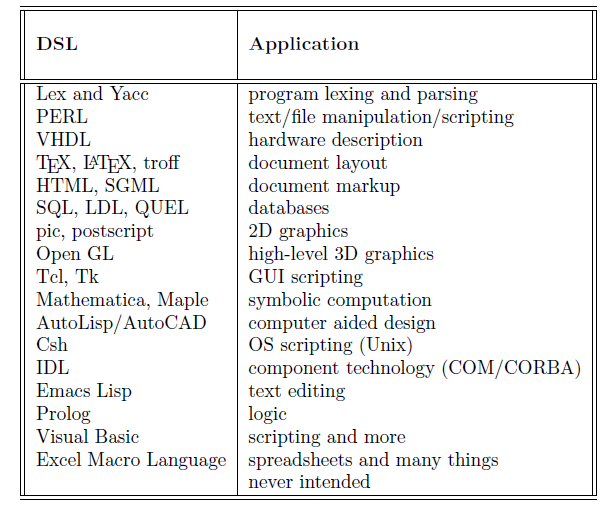
\includegraphics[scale=0.5]{Figures/dsl_table}
	\end{figure}	
\end{frame}


\end{document}